% Figure 1, horizontal variant: precompiled to figures/cascade_diagram.pdf (see README.md). Palatino (mathpazo) as
% in the article, natural size = width of the MDPI text column at most, lettering 8 to 9 pt; numbers from numbers.tex.
\documentclass[border=1pt]{standalone}
\usepackage[T1]{fontenc}
\usepackage{mathpazo}
\usepackage{tikz}
\usetikzlibrary{arrows.meta,positioning,shapes.geometric,fit,backgrounds,calc}
\input{numbers}
\definecolor{lite}{HTML}{08306B}
\definecolor{full}{HTML}{B2182B}
\begin{document}
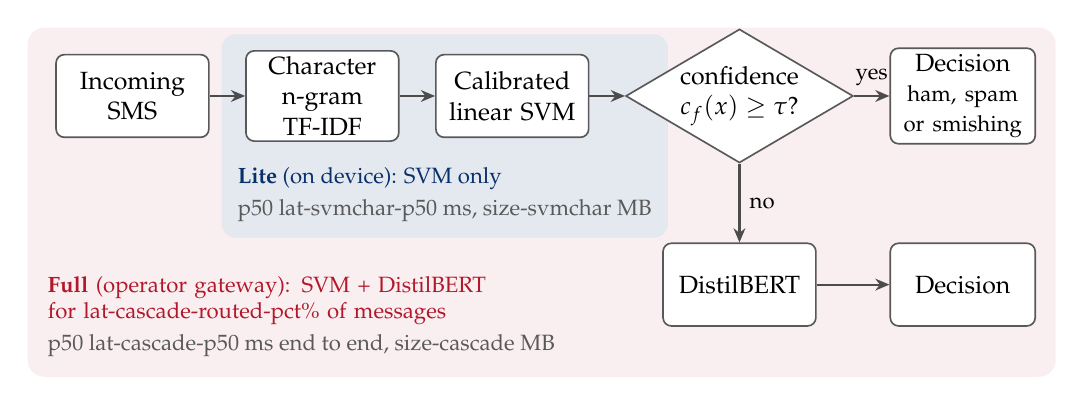
\begin{tikzpicture}[font=\small, node distance=4.5mm and 4.5mm,
  box/.style={draw=black!65, line width=0.6pt, rounded corners=3pt, fill=white, align=center,
              minimum height=10.5mm, text width=18mm, inner sep=2pt},
  dec/.style={draw=black!65, line width=0.6pt, diamond, aspect=1.7, fill=white, align=center, inner sep=0.5pt},
  arr/.style={-{Stealth[length=1.8mm,width=1.5mm]}, line width=0.75pt, draw=black!70},
  lab/.style={font=\footnotesize, align=left, anchor=north west, inner sep=0pt},
  num/.style={font=\footnotesize, text=black!65, align=left, anchor=north west, inner sep=0pt}]
\node[box] (sms) {Incoming\\SMS};
\node[box, right=of sms] (tfidf) {Character\\n-gram TF-IDF};
\node[box, right=of tfidf] (svm) {Calibrated\\linear SVM};
\node[dec, right=of svm] (d) {confidence\\$c_f(x)\ge\tau$?};
\node[box, right=of d, text width=17mm] (y1) {Decision\\{\footnotesize ham, spam}\\{\footnotesize or smishing}};
\node[box, below=10mm of d] (bert) {DistilBERT};
\node[box, text width=17mm] at (bert -| y1) (y2) {Decision};
\draw[arr] (sms) -- (tfidf);
\draw[arr] (tfidf) -- (svm);
\draw[arr] (svm) -- (d);
\draw[arr] (d) -- node[above, font=\footnotesize] {yes} (y1);
\draw[arr] (d) -- node[right, font=\footnotesize] {no} (bert);
\draw[arr] (bert) -- (y2);
% Lite: the character model alone; Full: the whole cascade
\node[lab, text=lite] (litelab) at ($(tfidf.south west)+(-1mm,-3.2mm)$) {\textbf{Lite} (on device): SVM only};
\node[num] (litenum) at ($(litelab.south west)+(0,-1mm)$) {p50 \val{lat-svmchar-p50}~ms, \val{size-svmchar}~MB};
\node[lab, text=full, text width=72mm] (fulllab) at ($(sms.south west)+(-1mm,-17.5mm)$)
  {\textbf{Full} (operator gateway): SVM + DistilBERT\\for \val{lat-cascade-routed-pct}\% of messages};
\node[num] (fullnum) at ($(fulllab.south west)+(0,-1mm)$) {p50 \val{lat-cascade-p50}~ms end to end, \val{size-cascade}~MB};
\begin{scope}[on background layer]
  \node[rounded corners=6pt, fill=full!7, inner sep=2.5mm, fit=(sms)(y1)(y2)(bert)(fullnum)(fulllab)] {};
  \node[rounded corners=5pt, fill=lite!11, inner sep=2mm, fit=(tfidf)(svm)(litelab)(litenum)] {};
\end{scope}
\end{tikzpicture}
\end{document}
